%% play.tex
%%

%% ==============================
\section{Play : Un langage d'Action}
\label{sec:play}
%% ==============================

%% question-6.tex
%%

%% ==============================
\subsection{Diagramme d'objet d'un niveau}
\label{sec:question-6}
%% ==============================

La propriété du jeu qui n'est pas satisfaite par ce niveau est celle de l'accesibilité du coffre par le joueur. En effet dans ce niveau, il n'est pas possible au joueur d'atteindre le coffre.

Le diagramme d'objet suivant décrit le niveau à la figure 3:

\begin{figure}[h!]
	\centering
	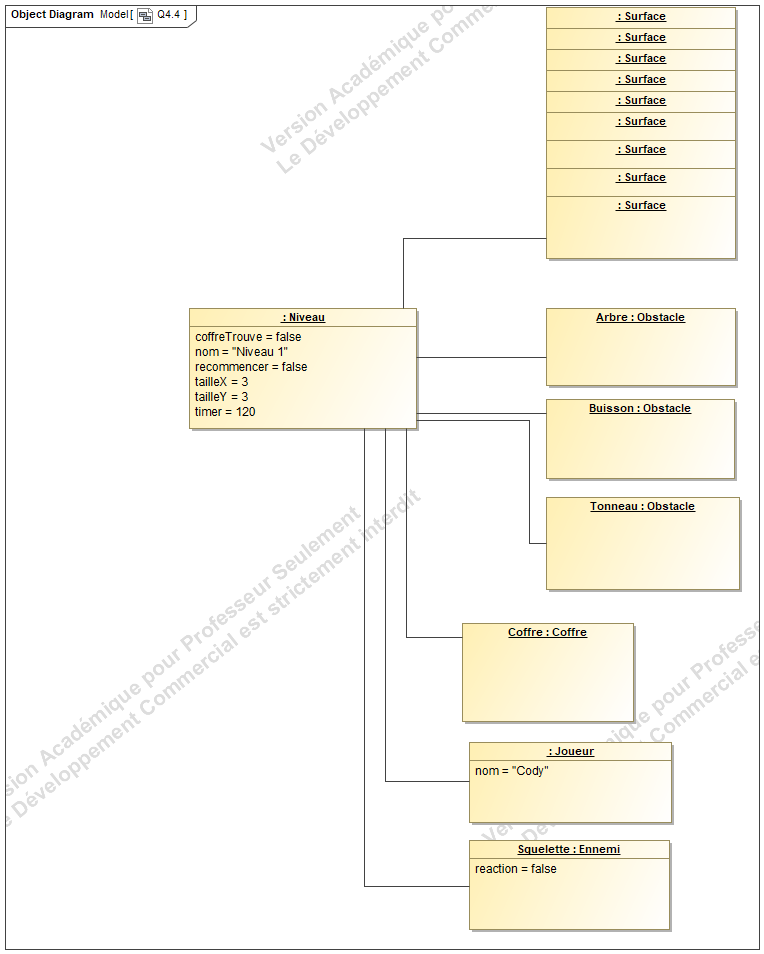
\includegraphics[width=350pt]{assets/Diagramme_objet}
	\caption{Diagramme d'objet de la figure 4.4}
	\label{fig:diagrammeobjet}
\end{figure}

\newpage
%% question-7.tex
%%

%% ==============================
\subsection{Modélisation du concept de stratégie}
\label{sec:question7}
%% ==============================
Voici un diagramme de classe qui fixe les éléments principaux d'une stratégie :

Une \emph{Stratégie} est composé d'une \emph{vision court terme} et une \emph{vision long terme} qui sont toutes les deux articulées par des objectifs eux même réalisés par des règles.

Une \emph{Stratégie} comporte également des \emph{Déclaration} pouvant être des modules ou des variables.

\begin{figure}[h!]
	\centering
	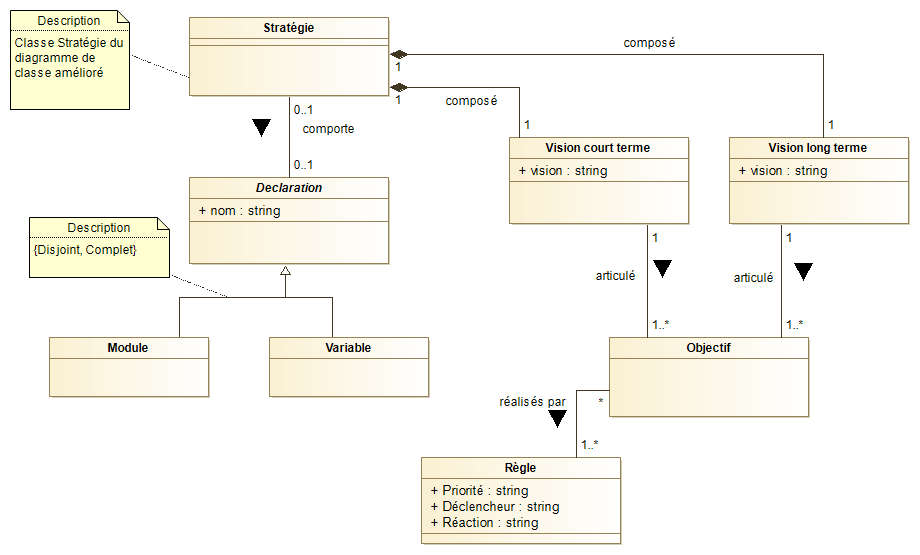
\includegraphics[width=450pt]{assets/strat_base}
	\caption{Diagramme de classe d'une stratégie}
	\label{fig:strategie}
\end{figure}

\newpage
%% question-8.tex
%%

%% ==============================
\subsection{Modélisation du concept de Type}
\label{sec:question8}
%% ==============================

Le concept de \emph{Type} est modélisé de la manière présentée à la figure \ref{fig:type}. La classe \emph{Type} est parent de plusieurs classes présentes dans ce diagramme \emph{Enumération}, \emph{TypePrimitif},\emph{Tableau}. 

On peut remarquer que le type \emph{void} n'est pas considéré comme un type primitif et est donc directement relié à la classe \emph{Type}. 

\begin{figure}
	\centering
	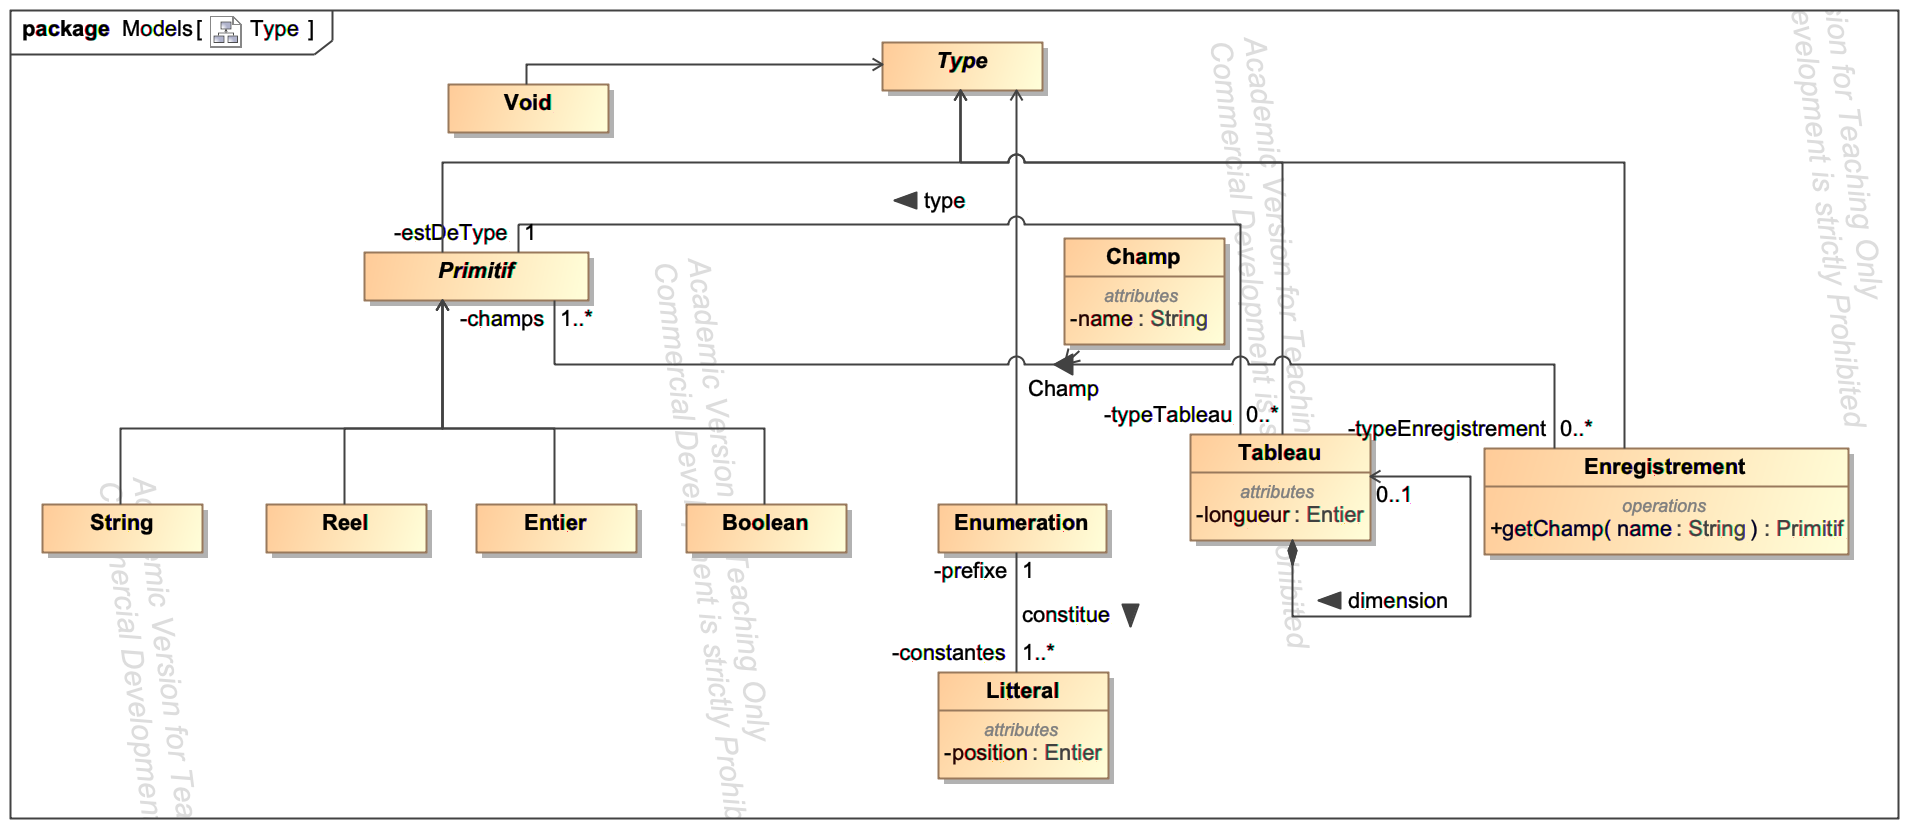
\includegraphics[width=500pt]{assets/class__Type}
	\caption{Diagramme de classe d'un type}
	\label{fig:type}
\end{figure}

%% question-9.tex
%%

%% ==============================
\subsection{Raffinement du concept d'Instruction}
\label{sec:question9}
%% ==============================

Présenté à la figure \ref{fig:instruction}, le raffinement d'\emph{Instruction} montre qu'une \emph{Instruction} possède trois enfants direct (\emph{Composée}, \emph{Affectation} et \emph{AppelProcédure}).

Le diagramme montre aussi qu'une Instruction est enfant de \emph{Déclaration} (comme présenté dans la figure \ref{fig:declaration}). Cela permet d'éviter d'avoir des tableaux de \emph{Void}.

Sur le diagramme, nous pouvons remarquer la classe \emph{Parametres}, celle-ci a été représentée dans la figure \ref{fig:declaration}.  

\begin{figure}
	\centering
	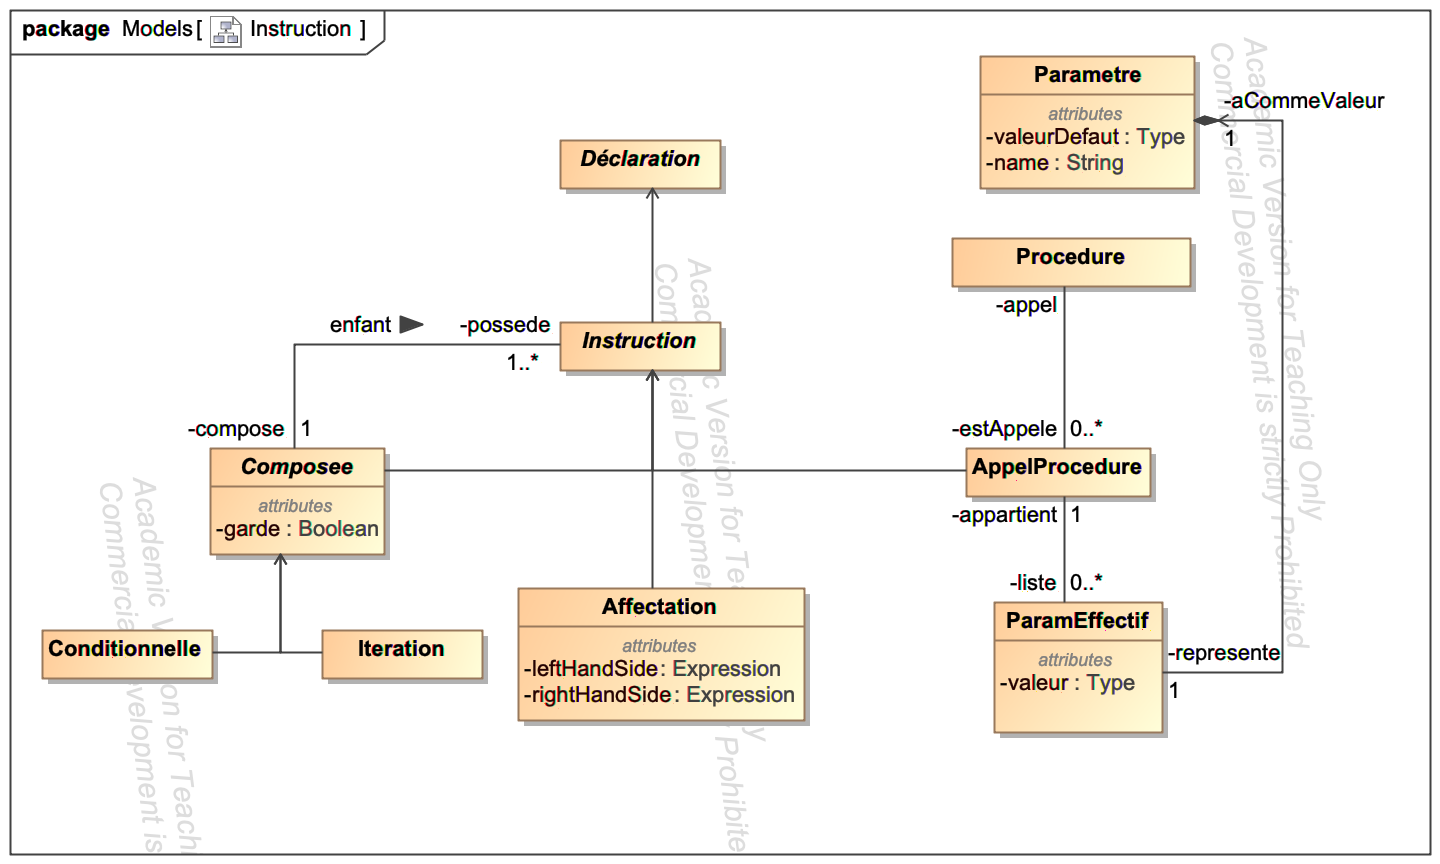
\includegraphics[width=500pt]{assets/class__Instruction}
	\caption{Diagramme de classe d'une instruction}
	\label{fig:instruction}
\end{figure}

%% question-10.tex
%%

%% ==============================
\subsection{Modélisation explicite d'un objectif}
\label{sec:question10}
%% ==============================

Le concept d'objectif est présenté à l'aide de la figure \ref{fig:objectif}. Un \emph{Objectif} est parent de 4 enfants : \emph{Neant} qui est l'objectif par défault. \emph{Combinable} qui est lui même parent de \emph{AllerVers}, \emph{Contourner} et \emph{Eviter}.
\emph{CollecterMax} et \emph{Combattre} sont les deux derniers enfants.
Les \emph{Objectif} sont réalisés par des règles qui possèdent des \emph{Reaction}.

\begin{figure}
	\centering
	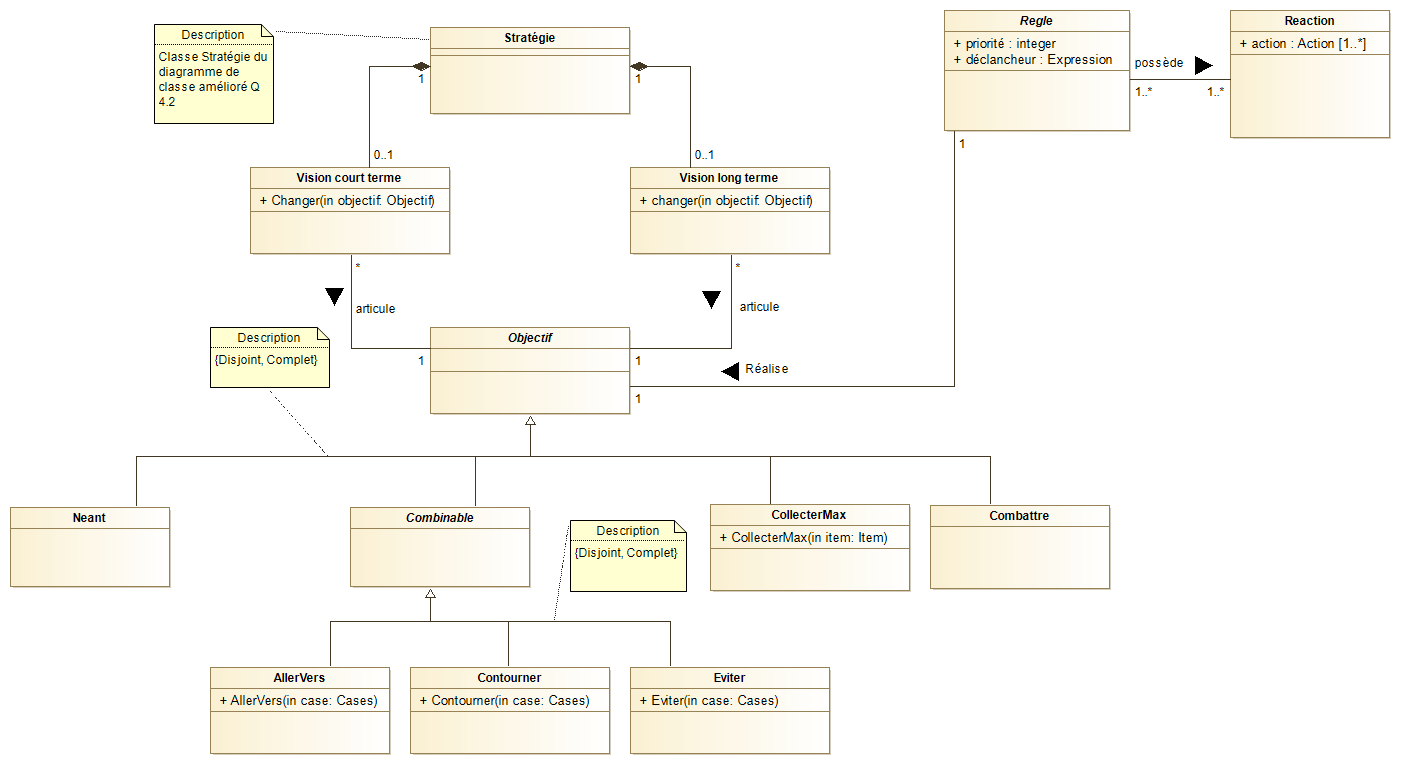
\includegraphics[width=500pt]{assets/class__Objectif}
	\caption{Diagramme de classe d'un objectif}
	\label{fig:objectif}
\end{figure}

%% question-11.tex
%%

%% ==============================
\subsection{Modélisation explicite d'une action}
\label{sec:question11}
%% ==============================

Le concept d'action est présenté à l'aide de la figure \ref{fig:action}. Une \emph{Action} est parent de 6 enfants : \emph{SeDeplacer}, \emph{UtiliserItem}, \emph{Revetir}, \emph{Frapper}, \emph{Tirer} et \emph{ConsulterRadar}.

C'est un personnage qui dispose de ces actions.

\begin{figure}
	\centering
	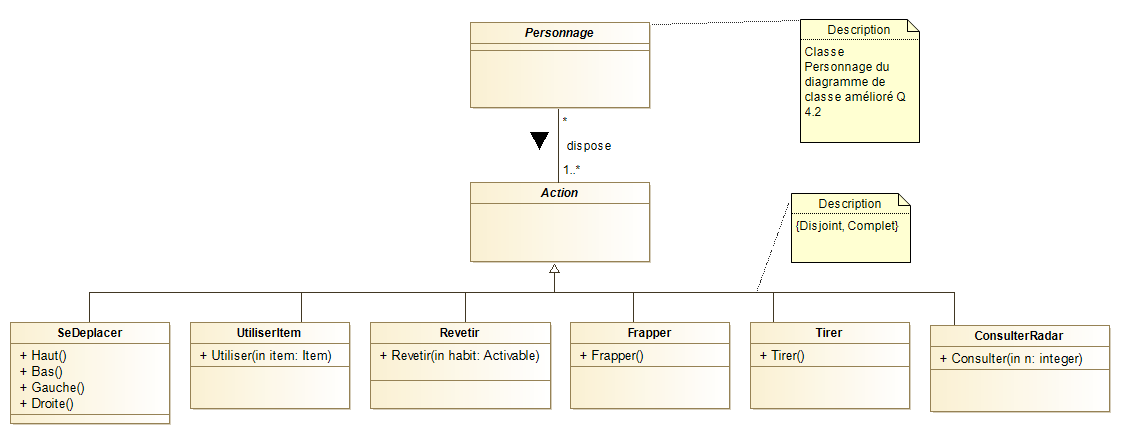
\includegraphics[width=500pt]{assets/class__Action}
	\caption{Diagramme de classe d'une action}
	\label{fig:action}
\end{figure}
%% question-12.tex
%%

%% ==============================
\subsection{Modélisation explicite d'une expression}
\label{sec:question12}
%% ==============================

Le concept d'expression est présenté à l'aide de la figure \ref{fig:expression}. Une \emph{Expression} contient une \emph{Parenthese} et peut prendre la forme de celle-ci. Une Expression peut aussi être un \emph{Literal} qui est une variable, une 
\emph{ExpressionGauche} qui elle même peut être un \emph{AppelVariable} qui invoque une variable, un \emph{AppelChamp} qui provient d'un \emph{Enregistrement}, un \emph{AppelCellule} qui a comme source un \emph{Tableau}. Une \emph{Expression} peut aussi être
un \emph{AppelModule} comportant des \emph{Parametre}, une \emph{Expression Unaire} ou \emph{Binaire} comportant des \emph{Operateur}.

\begin{figure}[h!]
	\centering
	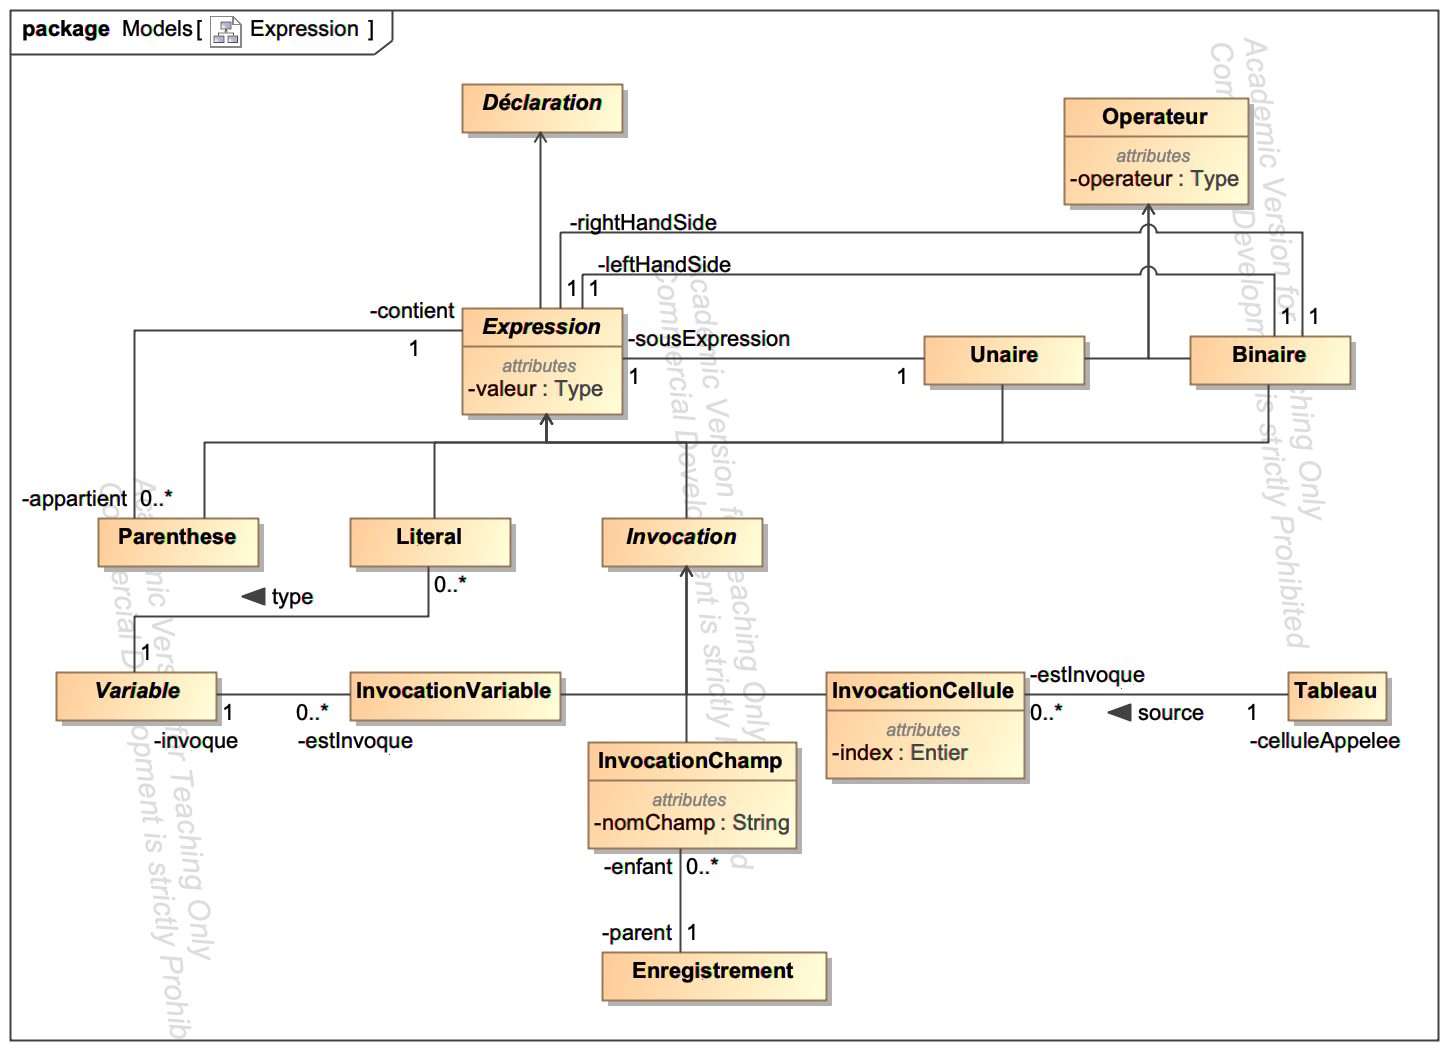
\includegraphics[width=450pt]{assets/class__Expression}
	\caption{Diagramme de classe d'une expression}
	\label{fig:expression}
\end{figure}

\newpage
%% question-13.tex
%%

%% ==============================
\subsection{\textsc{Ocl} - Contrats sur l'opération \emph{type(exp : Expression) : Type}}
\label{sec:question13}
%% ==============================

Dans les différents contrats, la fonction \emph{oclType()} est utilisée. Il s'agit d'une fonction fourni par OCL qui permet d'évaluer le type de l'instance sur laquelle il est appelé \citep{Omg2012}.

Le contrat OCL présenté ci-dessous (Listing \ref{lst:type_type}) spécifie que le type des littéraux est le type qui leur correspond.

\begin{lstlisting}[caption=Le type des littéraux est le type qui leur correspond,captionpos=b,label={lst:type_type},language=OCL]
context Expression::type(exp: Expression)
	post:
		if exp.oclIsTypeOf(Primitif) then
			return exp.oclType()
\end{lstlisting}

Le contrat du listing \ref{lst:type_unaire} indique que le type d'une expression unaire est lié au type de l'opérateur, à condition que sa sous-expression y corresponde.

\begin{lstlisting}[caption=Contrat OCL sur le type unaire,captionpos=b,label={lst:type_unaire},language=OCL]
context Expression::type(exp: Expression)
	post:
		if exp.oclIsTypeOf(Unaire) then
			if exp.operateur.oclIsTypeOf(
				exp.sous-expression.oclType()
			) then
				return exp.operateur.oclType()
\end{lstlisting}

Le contrat OCL suivant (Listing \ref{lst:type_binaire}) défini qu'un type d'une expression binaire est lié au type de son opérateur.

\begin{lstlisting}[caption=Contrat OCL sur le type binaire,captionpos=b,label={lst:type_binaire},language=OCL]
context Expression::type(exp: Expression)
	post:
		if exp.oclIsTypeOf(Binaire) then
			if exp.operateur.oclIsTypeOf(
				exp.leftHandSide.oclType()
			) and exp.operateur.oclIsTypeOf(
				exp.rightHandSide.oclType()
			) then
				return exp.operateur.oclType()
\end{lstlisting}

Le contrat ci-dessous (Listing \ref{lst:type_paranthese}) spécifie que le type d'une expression paranthésée est le type de sa sous-expression.

\begin{lstlisting}[caption=Contrat OCL sur le type parenthèsée,captionpos=b,label={lst:type_paranthese},language=OCL]
context Expression::type(exp: Expression)
	post:
		if exp.oclIsTypeOf(Parenthese) then
			return exp.sous-expression.oclType()
\end{lstlisting}

Le contrat suivant (Listing \ref{lst:type_record}) spécifie que le type d'une expression gauche correspondant à l'accès à un champ est le type de sa déclaration dans l'enregistrement.

\begin{lstlisting}[caption=Contrat OCL sur le type d'un enregistrement,captionpos=b,label={lst:type_record},language=OCL]
context Expression::type(exp: Expression)
	post:
		if exp.oclIsTypeOf(Binaire) then
			if exp.rightHandSide.oclIsTypeOf(InvocationChamp) then
				return exp.rightHandSide.parent
					.getChamp(exp.rightHandSide.nomChamp)
					.oclType()
\end{lstlisting}

Le dernier contrat présenté dans cette section (Listing \ref{lst:type_array}) spécifie que le type d'une expression gauche correspondant à l'accès à une case d'un tableau est le type de la déclaration du tableau.

\begin{lstlisting}[caption=Contrat OCL sur le type d'un tableau,captionpos=b,label={lst:type_array},language=OCL]
context Expression::type(exp: Expression)
	post:
		if exp.oclIsTypeOf(Binaire) then
			if exp.rightHandSide.oclIsTypeOf(InvocationCellule) then
				return exp.rightHandSide.source.type.oclType()
\end{lstlisting}

%% question-14.tex
%%

%% ==============================
\subsection{\textsc{Ocl} - Contraintes d'unicité}
\label{sec:question14}
%% ==============================

La première contrainte d'unicité sur le nom unique des modules est spécifiée comme suit :

\begin{lstlisting}[caption=Nom unique au sein d'une stratégie,captionpos=b,label={lst:nom_unique},language=OCL]
context Strategie inv nomUnique :
	if self.Declaration.allInstances -> oclIsTypeOf(Module) and
		self.Declaration.forall( m1, m2 | m1.nom <> m2.nom)
	then
		true
	else
		false
	endif
\end{lstlisting}

La contrainte sur le nom des variables globales est la suivante :

\begin{lstlisting}[caption=Nom unique d'une variable globale,captionpos=b,label={lst:unique_globale},language=OCL]
context Strategie inv nomVarGlobal :
	if self.Declaration.allInstances ->oclIsTypeOf(Variable) and
		self.Declaration.forall( v1,v2 | v1.nom <> v2.nom)
	then
		true
	else
		false
	endif
\end{lstlisting}

La contrainte sur les variables locales est la suivante :

\begin{lstlisting}[caption=Nom unique des variables locales,captionpos=b,label={lst:nom_locale},language=OCL]
context Module inv uniqueLocale :
	self.Variable.allInstances -> forall(v1,v2 | 
	v1.nom <> v2.nom implies v1 <> v2)
\end{lstlisting}

La contrainte sur les noms des paramètres d'un module est la suivante :

\begin{lstlisting}[caption=Nom unique des paramètres,captionpos=b,label={lst:unique_param},language=OCL]
context Module inv uniqueParam :
	self.Parametre.allInstances -> forall(p1,p2 | 
	p1.nom <> p2.nom implies p1 <> p2)
\end{lstlisting}

La contrainte sur le nom des types soit globalement unique est la suivante :

\begin{lstlisting}[caption=Nom unique des types,captionpos=b,label={lst:type_unique},language=OCL]
context Type inv difNom :
	self.allInstances -> forall( e,t | 
	e.oclIsTypeOf(Enumeration) and t.oclIsTypeOf(Tableau) 
	and e.nom <> t.nom)
\end{lstlisting}
%% question-15.tex
%%

%% ==============================
\subsection{\textsc{Ocl} - Contrats sur l'opération \emph{prec\_mouv() : Déplacement}}
\label{sec:question15}
%% ==============================

Le premier contract OCL (Listing \ref{lst:action_move}) va permet de vérifier que lors d'un déplacement, si on tente d'accéder à une case ou se trouve un obstacle, le déplacement n'est pas effectué.

 \begin{lstlisting}[caption=On empêche le déplacement si la case est occupée par un obstacle,captionpos=b,label={lst:action_move},language=OCL]
context ProcedureAction::right()
	def: player = NiveauEnCours::elements.select(e -> e.name == "Cody"
					and e.oclIsTypeOf(Player))
	post rightObstacle:
		if 	NiveauEnCours::getElementAtPosition(player.Position.X + 1, 
			player.Position.Y).oclIsTypeOf(Obstacle) then
			player.Position.X == player.Position.X@pre and
			player.Position.Y == player.Position.Y@pre
			
context ProcedureAction::left()
	def: player = NiveauEnCours::elements.select(e -> e.name == "Cody"
					and e.oclIsTypeOf(Player))
	post leftObstacle:
		if 	NiveauEnCours::getElementAtPosition(player.Position.X - 1, 
			player.Position.Y).oclIsTypeOf(Obstacle) then
			player.Position.X == player.Position.X@pre and
			player.Position.Y == player.Position.Y@pre
			
context ProcedureAction::up()
	def: player = NiveauEnCours::elements.select(e -> e.name == "Cody"
					and e.oclIsTypeOf(Player))
	post upObstacle:
		if 	NiveauEnCours::getElementAtPosition(player.Position.X , 
			player.Position.Y - 1).oclIsTypeOf(Obstacle) then
			player.Position.X == player.Position.X@pre and
			pPlayer.Position.Y == player.Position.Y@pre
			
context ProcedureAction::down()
	def: player = NiveauEnCours::elements.select(e -> e.name == "Cody"
					and e.oclIsTypeOf(Player))
	post downObstacle:
		if 	NiveauEnCours::getElementAtPosition(player.Position.X, 
			player.Position.Y + 1).oclIsTypeOf(Obstacle) then
			player.Position.X == player.Position.X@pre and
			player.Position.Y == player.Position.Y@pre
\end{lstlisting}

Le contrat OCL (Listing \ref{lst:action_tunnel}) suivant indique que si le joueur accède à une case ou ce trouve un tunnel, il ressort dans la case suivant le dernier mouvement à partir de l'autre tunnel.

\begin{lstlisting}[caption=Contract OCL pour le passage dans un tunnel,captionpos=b,label={lst:action_tunnel},language=OCL]
context ProcedureAction::right()
	def: tunnel : Position
	def: player = NiveauEnCours::elements.select(e -> e.name == "Cody"
					and e.oclIsTypeOf(Player))
	post:
		tunnel = NiveauEnCours::getElementAtPosition(
		player.PositionX + 1, Player.PositionY)
			
		if tunnel.oclIsTypeOf(Tunnel) then
			player.Position.X == tunnel.Sortie.X + 1 
			and player.Position.Y == tunnel.Sortie.Y

context ProcedureAction::left()
	def: tunnel : Position
	def: player = NiveauEnCours::elements.select(e -> e.name == "Cody"
					and e.oclIsTypeOf(Player))
	post:
		tunnel = NiveauEnCours::getElementAtPosition(
		player.PositionX - 1, Player.PositionY)
			
		if tunnel.oclIsTypeOf(Tunnel) then
			player.Position.X == tunnel.Sortie.X - 1
			and player.Position.Y == tunnel.Sortie.Y
			
context ProcedureAction::up()
	def: tunnel : Position
	def: player = NiveauEnCours::elements.select(e -> e.name == "Cody"
					and e.oclIsTypeOf(Player))
	post:
		tunnel = NiveauEnCours::getElementAtPosition(
		player.PositionX, Player.PositionY - 1)
			
		if tunnel.oclIsTypeOf(Tunnel) then
			player.Position.X == tunnel.Sortie.X and
			player.Position.Y == tunnel.Sortie.Y - 1

context ProcedureAction::down()
	def: tunnel : Position
	def: player = NiveauEnCours::elements.select(e -> e.name == "Cody"
					and e.oclIsTypeOf(Player))
	post:
		tunnel = NiveauEnCours::getElementAtPosition(
		player.PositionX, Player.PositionY + 1)
			
		if tunnel.oclIsTypeOf(Tunnel) then
			player.Position.X == tunnel.Sortie.X and
			player.Position.Y == tunnel.Sortie.Y + 1
\end{lstlisting}

Enfin, le dernier contract OCL (Listing \ref{lst:action_jump}) permet d'indiquer que si le joueur saute, il atterit deux cases plus loin dans la même direction. Par contre, s'il y a un obstacle deux cases plus loin, le joueur ne bouge pas.

\begin{lstlisting}[caption=Contract OCL psur le saut,captionpos=b,label={lst:action_jump},language=OCL]
context ProcedureAction::jump()
	def: newPosition : Position
	def: player = Niveau::elements.select(e -> e.name == "Cody" and
					e.oclIsTypeOf(Player))
	post:
		if prec_mouv() == right then
			newPosition = NiveauEnCours::getElementAtPosition(
			player.PositionX + 2, player.PositionY)
			
			if newPosition.oclIsTypeOf(Surface) then
				player.Position.X == player.Position.X@pre + 2 
				and player.Position.Y == player.Position.Y@pre
			else
				player.Position.X == player.Position.X@pre 
				and player.Position.Y == player.Position.Y@pre
		if prec_mouv() == left then
			newPosition = NiveauEnCours::getElementAtPosition(
			player.PositionX - 2, player.PositionY)
			
			if newPosition.oclIsTypeOf(Surface) then
				player.Position.X == player.Position.X@pre - 2 
				and player.Position.Y == player.Position.Y@pre
			else		
				player.Position.X == player.Position.X@pre 
				and player.Position.Y == player.Position.Y@pre
		if prec_mouv() == up then
			newPosition = NiveauEnCours::getElementAtPosition(
			player.PositionX, player.PositionY - 2)
			
			if newPosition.oclIsTypeOf(Surface) then
				player.Position.X == player.Position.X@pre
				and player.Position.Y == player.Position.Y@pre
			else
				player.Position.X == player.Position.X@pre 
				and player.Position.Y == player.Position.Y@pre - 2
		if prec_mouv() == down then
			newPosition = NiveauEnCours::getElementAtPosition(
			player.PositionX, player.PositionY + 2)
			
			if newPosition.oclIsTypeOf(Surface) then
				player.Position.X == player.Position.X@pre 
				and player.Position.Y == player.Position.Y@pre + 2
			else
				player.Position.X == player.Position.X@pre 
				and player.Position.Y == player.Position.Y@pre
\end{lstlisting}
%% question-16.tex
%%

%% ==============================
\subsection{\textsc{Ocl} - Contrats sur l'opération \emph{Expression :: type() : Type}
\label{sec:question16}
%% ==============================

Ce premier contrat porte sur le fait que le type du litéral retourné corresponde au litéral :

\begin{lstlisting}[caption=Contrat \textsc{Ocl} sur le type des litéraux,captionpos=b,label={lst:type_literal},language=OCL]
context Expression :: type() : Type
	post:
		if Type.oclIsTypeOf(TypePrimitif) then
			return Type.oclType()
\end{lstlisting}

Le contrat sur l'opérateur unaire est la suivante :

\begin{lstlisting}[caption=Contrat \textsc{Ocl} sur le type unaire,captionpos=b,label={lst:type_unaire},language=OCL]
context Expression :: type() : Type
	post:
		if Type.oclIsTypeOf(Unaire) then
			if Type.operateur.oclIsTypeOf(
				Type.sous-expression.oclType()
			) then
				return Type.operateur.oclType()
\end{lstlisting}

Le contrat correspondant à l'opérateur binaire est le suivant :

\begin{lstlisting}[caption=Contrat \textsc{Ocl} sur le type binaire,captionpos=b,label={lst:type_binaire},language=OCL]
context Expression :: type() : Type
	post:
		if Type.oclIsTypeOf(Binaire) then
			if Type.operateur.oclIsTypeOf(
				Type.leftHandSide.oclType()
			) and Type.operateur.oclIsTypeOf(
				Type.rightHandSide.oclType()
			) then
				return Type.operateur.oclType()
\end{lstlisting}

Le contrat sur le type de la sous-expression dans une parenthèse est le suivant :

\begin{lstlisting}[caption=Contrat \textsc{Ocl} sur le type paranthésée,captionpos=b,label={lst:type_paranthese},language=OCL]
context Expression :: type() : Type
	post:
		if Type.oclIsTypeOf(Parenthese) then
			return Type.sous-expression.oclType()
\end{lstlisting}

Le contrat sur le type de la déclaration est le suivant :

Le contrat sur le type de renvoi d'une énumération de litéraux est le suivant :

\begin{lstlisting}[caption=Contrat \textsc{Ocl} sur le type de renvoi d'une énum de litéraux,captionpos=b,label={lst:type_énum},language=OCL]
context Expression :: type() : Type
	post :
		if Type.oclIsTypeOf(Litteral)
		then
			return
				Type.est.oslType()
\end{lstlisting}

Le contrat sur le type de retour d'un champ est le suivant :

\begin{lstlisting}[caption=Contrat \textsc{Ocl} sur le type de retour d'un champ,captionpos=b,label={lst:type_champ},language=OCL]
context Expression :: type() : Type
	post :
		if Type.oclIsTypeOf(Champ)
		then
			return
			Type.TypePrimitif.oclType()
\end{lstlisting}

Le contrat sur le type du contenu d'un tableau est le suivant :

\begin{lstlisting}[caption=Contrat \textsc{Ocl} sur le type de retour d'un tableau,captionpos=b,label={lst:type_tableau},language=OCL]
context Expression :: type() : Type
	post :
		if Type.oclIsTypeOf(Tableau)
		then
		 return
		 	Type.est.oclType()
\end{lstlisting}
%% %% question-17.tex
%%

%% ==============================
\subsection{Opération estTraversableGraceAuxItems() : Boolean}
\label{sec:question17}
%% ==============================

La classe de notre diagramme qui pourrait contenir cette opération est Case.

Le contrat de cette définition est le suivant :

\begin{lstlisting}[caption=Contrat \textsc{Ocl} sur l'opération estTraversableGraceAuxItems,captionpos=b,label={lst:operation},language=OCL]
context estTraversableGraceAuxItems(Case,Avatar) : Boolean :
    post :
        if Case.oclIsTypeOf(Zone) and (
            Case.aspect = Feu and
            Avatar.Inventaire.Objet.allInstances() ->
                forall(o | o.oclIsTypeOf(Bottes Pare-Feu))
            or
            Case.aspect = Eau and
            Avatar.Inventaire.Objet.allInstances() ->
                forall(o | o.oclIsTypeOf(Kit De Plongee))
            or
            Case.aspect = Glace and
            Avatar.Inventaire.Objet.allInstances() ->
                forall(o | o.oclIsTypeOf(Bottes a crampon))
        )
        then
            return true
        endif

\end{lstlisting}
